\documentclass[conference]{IEEEtran}
\IEEEoverridecommandlockouts
% The preceding line is only needed to identify funding in the first footnote. If that is unneeded, please comment it out.
%Template version as of 6/27/2024

\usepackage{cite}
\usepackage{amsmath,amssymb,amsfonts}
\usepackage{algorithmic}
\usepackage{graphicx}
\usepackage{float}
\usepackage{textcomp}
\usepackage{xcolor}
\usepackage[utf8]{inputenc}
\usepackage[spanish,es-tabla]{babel}
\usepackage{listings} 
\usepackage{setspace}

\def\BibTeX{{\rm B\kern-.05em{\sc i\kern-.025em b}\kern-.08em
    T\kern-.1667em\lower.7ex\hbox{E}\kern-.125emX}}


% --- CONFIGURACIÓN DE COLORES PARA EL CÓDIGO ---
\definecolor{fondoCodigo}{rgb}{0.95,0.95,0.92}
\definecolor{comentario}{rgb}{0.5,0.5,0.5}
\definecolor{palabraClave}{rgb}{0.0,0.0,0.8}
\definecolor{cadena}{rgb}{0.0,0.6,0.0}

\lstdefinestyle{estiloPython}{
    backgroundcolor=\color{fondoCodigo},   
    commentstyle=\color{comentario}\itshape,
    keywordstyle=\color{palabraClave}\bfseries,
    numberstyle=\tiny\color{comentario},
    stringstyle=\color{cadena},
    basicstyle=\ttfamily\footnotesize,
    breakatwhitespace=false,         
    breaklines=true,                 
    captionpos=b,                    
    keepspaces=true,                 
    numbers=left,                    
    numbersep=5pt,                  
    showspaces=false,                
    showstringspaces=false,
    showtabs=false,                  
    tabsize=4,
    frame=lines % Pone dos líneas elegantes arriba y abajo
}
\lstset{style=estiloPython}

\begin{document}

\title{Aprendiendo a jugar a Otelo: Agente Inteligente con Búsqueda Adversaria y Deep Learning}

\author{\IEEEauthorblockN{1\textsuperscript{st} Javier Luque Ruiz}
\IEEEauthorblockA{\textit{Grado en Ingeniería Informática - Ingeniería del Software} \\
\textit{Universidad de Sevilla}\\
Sevilla, España \\
javluqrui@alum.us.es}
}

\maketitle
\thispagestyle{plain} 
\pagestyle{plain}

\begin{abstract}
En este trabajo se presenta el desarrollo de un agente inteligente para el clásico juego de tablero Otelo (Reversi). El objetivo principal 
ha sido construir un sistema capaz de tomar decisiones estratégicas mediante la implementación del algoritmo clásico de Minimax con poda 
alfa-beta para explorar eficientemente el árbol de decisiones. Adicionalmente, se ha integrado una red neuronal profunda entrenada mediante 
autojuego para proporcionar una heurística de evaluación dinámica de las posiciones intermedias, reemplazando así las funciones de evaluación 
manuales clásicas y dotando al agente de la capacidad de deducir patrones espaciales.
\end{abstract}

\begin{IEEEkeywords}
Inteligencia Artificial, Otelo, Reversi, Minimax, Poda Alfa-Beta, Deep Learning, Python.
\end{IEEEkeywords}

\section{Introducción}
El desarrollo de agentes inteligentes capaces de tomar decisiones estratégicas en juegos de tablero ha sido uno de los grandes hitos históricos 
de la Inteligencia Artificial. Inspirado en los éxitos recientes de sistemas basados en aprendizaje profundo, este trabajo explora la combinación 
de algoritmos de búsqueda clásica bidireccional con técnicas modernas de redes neuronales artificiales.\\

El objetivo principal de este proyecto es construir un agente inteligente altamente competitivo para el clásico juego de Otelo. 
Específicamente, se aborda el diseño e implementación de un motor lógico eficiente, respaldado por el \textbf{algoritmo Minimax} con optimización de poda alfa-beta 
para explorar el inmenso espacio de estados del juego. La aportación central del sistema consiste en la hibridación de este algoritmo determinista con 
modelos paramétricos: se sustituyen las funciones heurísticas manuales por una red neuronal profunda, la cual ha aprendido a evaluar de forma autónoma 
la viabilidad de los estados intermedios basándose en un conjunto de datos masivo generado mediante técnicas de autojuego.\\

El resto del documento se estructura de la siguiente manera: la \textit{Sección II} detalla los fundamentos teóricos del juego y las bases algorítmicas; la 
\textit{Sección III} describe el diseño arquitectónico y la implementación del motor, el agente y las redes neuronales; la \textit{Sección IV} recoge el análisis 
empírico y los resultados de los torneos automatizados; finalmente, en las \textit{Secciones V y VI} se exponen las conclusiones obtenidas, posibles líneas 
de trabajo futuro y el uso de herramientas de asistencia generativa.

\section{Preeliminares}
\subsection{El juego de Otelo}
Otelo es un juego de estrategia de suma cero con información perfecta para dos jugadores, el cual se disputa sobre un tablero de $8 \times 8$ casillas, siguiendo el reglamento oficial de la Federación Mundial de Otelo \cite{otelo_rules}. 
La partida inicializa con una disposición central de cuatro fichas cruzadas (dos blancas y dos negras), cediendo el primer movimiento al jugador con las piezas negras.\\

\begin{figure}[H]
    \centering
    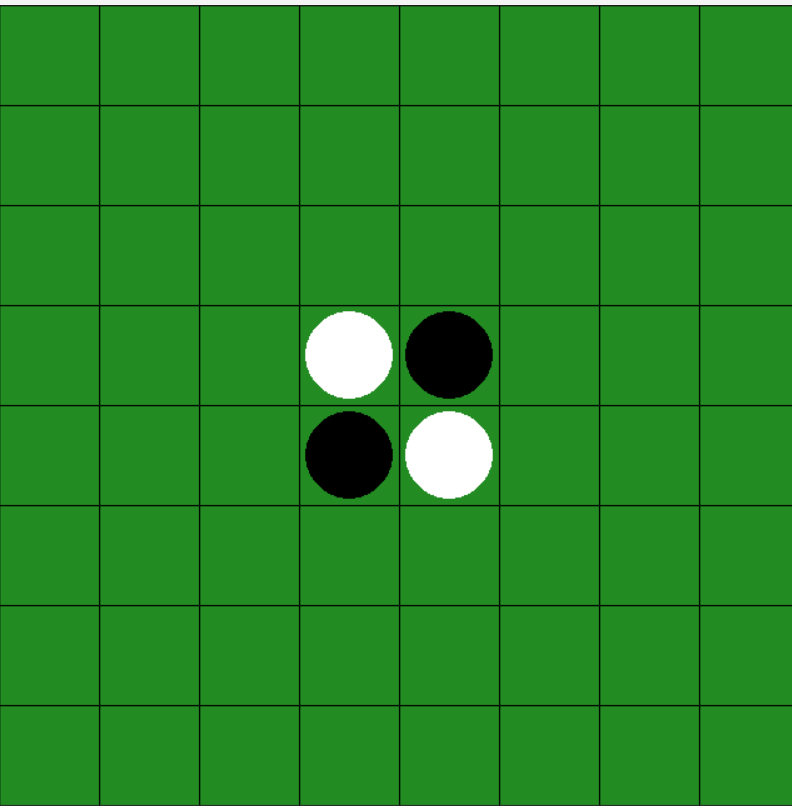
\includegraphics[width=0.65\columnwidth]{images/otelo-posicioninicial.png}
    \caption{Tablero inicial de Otelo con la disposición central de fichas.}
    \label{fig:otelo_board}
\end{figure}

La mecánica central del juego es el \textbf{flanqueo}: un movimiento legal consiste en colocar una ficha en una casilla vacía de forma que, 
en línea recta (horizontal, vertical o diagonal), una o más piezas del oponente queden atrapadas entre la nueva ficha y otra pieza del 
jugador activo. Las fichas flanqueadas son capturadas y cambian de color. \\

Para ilustrar esta mecánica, la Fig.~ \ref{fig:ejemplo-movimientos} muestra las casillas vacías donde el jugador con fichas negras puede colocar su pieza en el primer 
turno de la partida. Cada una de estas posiciones permite flanquear al menos una ficha blanca, cumpliendo así con la regla de legalidad del movimiento. Por el contrario, las casillas 
marcadas en rojo representan un movimiento ilegal, ya que, aunque estén adyacentes a fichas del oponente, colocar una ficha ahí no lograría atrapar ninguna ficha blanca entre dos fichas negras.

\begin{figure}[H]
    \centering
    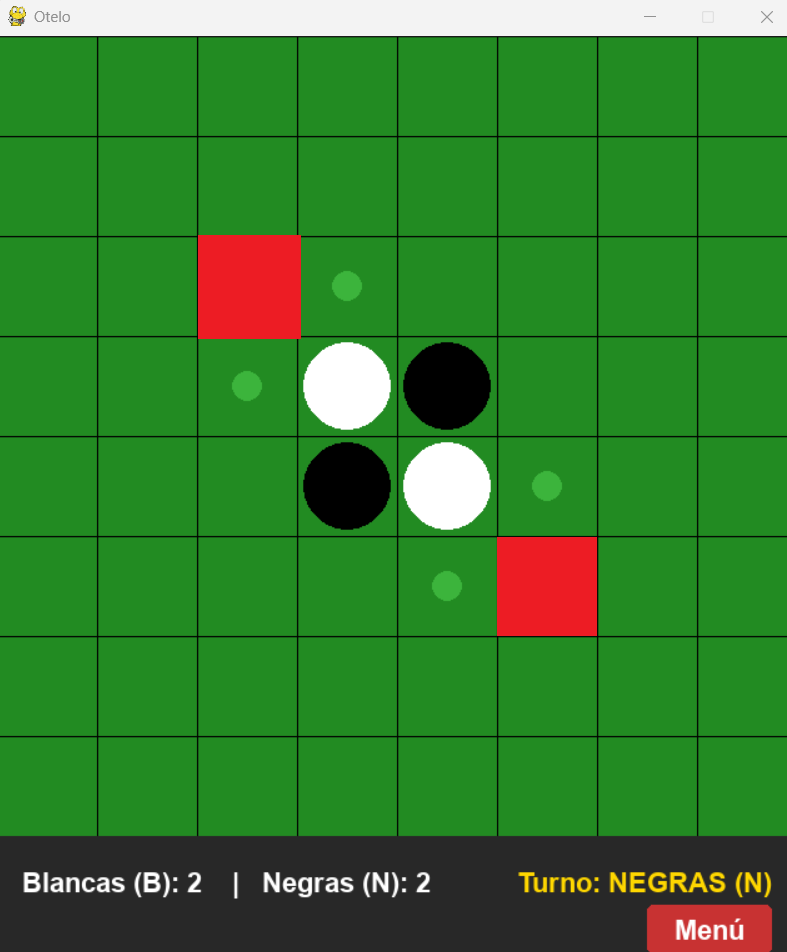
\includegraphics[width=0.65\columnwidth]{images/otelo-movimientos-validos.png}
    \caption{Ejemplo de movimientos: flanqueo válido (verde) y movimiento ilegal (rojo).}
    \label{fig:ejemplo-movimientos}
\end{figure}

Siguiendo con el escenario planteado, supongamos que el jugador de piezas negras decide ejecutar el movimiento válido situado más a la izquierda del tablero. Al colocar su 
ficha en esa posición, logra atrapar una pieza blanca del oponente contra otra de sus propias fichas negras situadas en el centro.\\

Como dicta la regla del flanqueo, esta ficha blanca es capturada y revertida al color negro. El resultado de esta acción se ilustra en la Fig.~\ref{fig:movimiento-ejecutado}. 
Tras este cambio en el tablero, el turno pasa inmediatamente al jugador de piezas blancas, continuando así el flujo natural de la partida.

\begin{figure}[H]
    \centering
    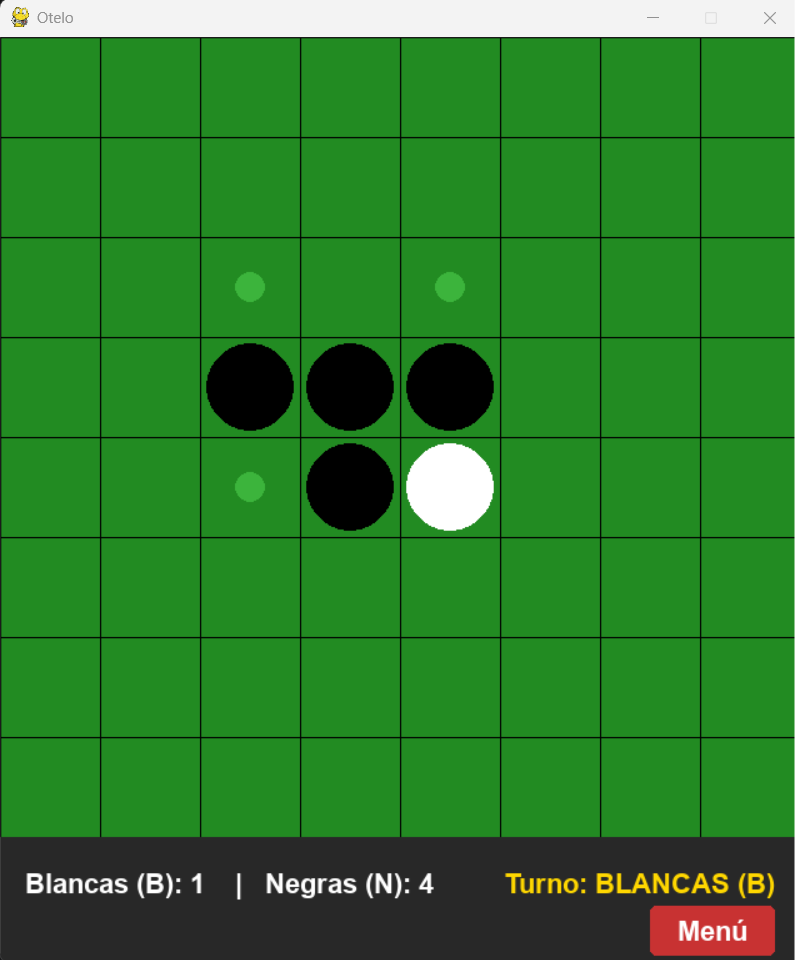
\includegraphics[width=0.65\columnwidth]{images/resultado-movimiento.png}
    \caption{Estado del tablero tras ejecutar el flanqueo. La ficha blanca capturada cambia a color negro.}
    \label{fig:movimiento-ejecutado}
\end{figure}

Esta restricción de movimientos obliga a los jugadores a desarrollar \textbf{estrategias de posicionamiento} a largo plazo. En este sentido, el control de las 
esquinas del tablero resulta vital, ya que una ficha colocada en una de las cuatro esquinas jamás podrá ser flanqueada por el oponente, garantizando su 
permanencia hasta el final de la partida. Del mismo modo, limitar la movilidad del rival (reduciendo sus opciones legales) es una táctica fundamental para 
forzarle a realizar movimientos perjudiciales.\\

Si en algún momento un jugador carece de movimientos legales que cumplan esta regla de flanqueo, está obligado a pasar su turno. La partida concluye cuando el 
tablero se llena o ningún jugador puede realizar un movimiento válido, resultando ganador aquel con mayor número de fichas de su color.\\

\subsection{Búsqueda Adversaria y Poda Alfa-Beta}
El desarrollo de un agente capaz de competir en juegos de tablero bidireccionales y de suma cero se fundamenta tradicionalmente en la 
teoría de la \textbf{búsqueda adversaria} \cite{russell}. En este contexto, 
el algoritmo Minimax constituye la técnica esencial para modelar la toma de decisiones estratégicas. 
Este enfoque asume que ambos jugadores 
actúan de forma completamente óptima bajo roles contrapuestos: el agente 
inteligente adopta el rol de maximizador (MAX), cuyo objetivo es seleccionar el movimiento que maximice su recompensa final, mientras que el oponente 
actúa como minimizador (MIN), intentando reducir a toda costa el beneficio de MAX.\\

El proceso opera de forma recursiva construyendo un árbol de juego, donde los nodos representan los estados del tablero y las aristas corresponden a los 
movimientos legales posibles. Los valores de utilidad se calculan desde los nodos terminales (hojas) y se propagan hacia arriba a través de los niveles 
del árbol: un nodo en un nivel MAX heredará el valor máximo de sus hijos, mientras que un nodo en un nivel MIN heredará el valor mínimo.\\

Sin embargo, el espacio de estados de Otelo es masivo, con un factor de ramificación medio elevado. Explorar el árbol completo hasta el final de la partida 
desde los primeros turnos es computacionalmente inabarcable en tiempo real. Por ello, se implementa una estrategia de búsqueda con \textbf{corte de profundidad} (\textit{cutting-off search}). 
Al alcanzar un límite preestablecido de niveles (profundidad $d$), la simulación se detiene de manera controlada y se invoca una función heurística de evaluación numérica. Esta 
función estima de forma estática la calidad de la posición actual del tablero para MAX, sustituyendo el valor de utilidad real del fin de la partida.\\

Para mitigar el coste computacional y permitir exploraciones más profundas en menores tiempos de respuesta, se integra la optimización de la \textbf{poda alfa-beta}. 
Esta técnica mantiene el control de los peores escenarios asumibles por cada jugador durante la exploración recursiva mediante dos variables adaptativas:
\begin{itemize}
    \item $\alpha$: Representa la mejor opción (el valor más alto) que el jugador MAX ha logrado asegurar hasta el momento a lo largo del camino de búsqueda.
    \item $\beta$: Representa la mejor opción (el valor más bajo) que el jugador MIN ha conseguido asegurar hasta el momento.
\end{itemize}

A medida que el algoritmo recorre el árbol en profundidad, actualiza estos valores. La poda (o descarte matemático de ramas) se ejecuta inmediatamente 
en el momento en que se cumple la condición:
\begin{equation}
    \alpha \ge \beta
\end{equation}

Esta desigualdad implica que el jugador actual puede forzar un resultado mejor en otra rama previamente explorada, por lo que el oponente ideal 
jamás permitiría alcanzar el estado actual. Descartar estas ramas irrelevantes reduce drásticamente el número de nodos evaluados sin alterar en absoluto 
el movimiento óptimo final que devolvería el algoritmo Minimax puro.\\

Para comprender visualmente este proceso de descarte, la Fig ~\ref{fig:alfa-beta} ilustra el escenario conceptual diseñado para el árbol de decicisión. Como se 
puede observar, tras evaluar el primer hijo de un nodo MIN y obtener un valor que resulta inferior o igual al valor $\alpha$ asegurado por MAX, se activa inmediatamente 
el criterio de poda, omitiendo la exploración de los nodos restantes (marcados con un descarte explícito).

\begin{figure}[H]
    \centering
    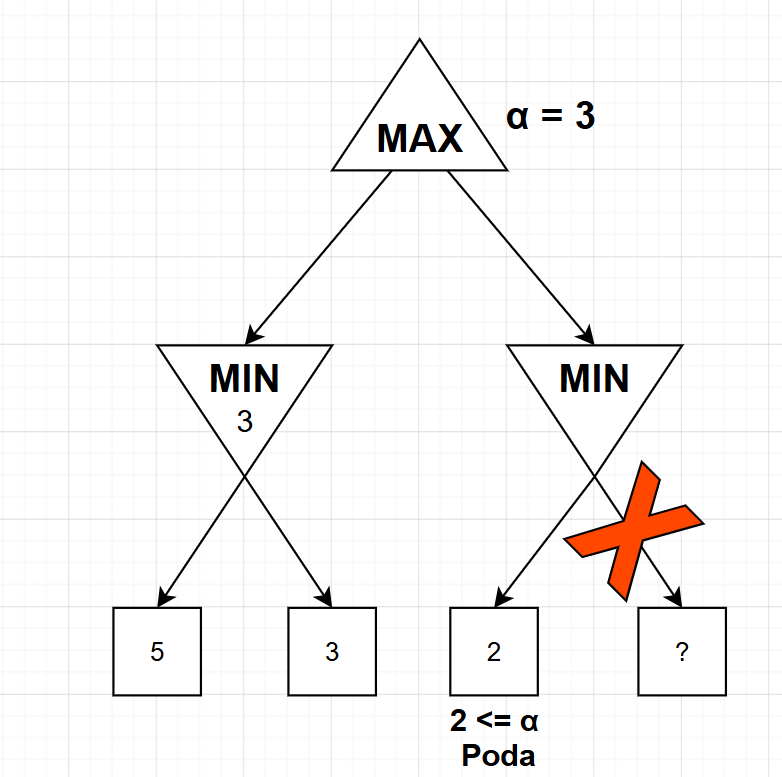
\includegraphics[width=0.9\columnwidth]{images/arbol-minimax.png}
    \caption{Ejemplo conceptual de poda alfa-beta en un árbol de búsqueda. Los nodos descartados se marcan con una cruz roja, indicando que no se evaluarán debido a la condición $\alpha \ge \beta$.}
    \label{fig:alfa-beta}
\end{figure}

\subsection{Redes Neuronales y Deep Learning}
Las redes neuronales artificiales son modelos computacionales inspirados en la estructura y el funcionamiento del cerebro 
humano, diseñados para aproximar funciones matemáticas complejas a partir de datos empíricos \cite{goodfellow}. En particular, 
las redes con alimentación hacia adelante (\textit{feedforward neural networks}) se estructuran mediante unidades básicas denominadas \textbf{neuronas}, 
las cuales se organizan en capas secuenciales (entrada, ocultas y salida) \cite{apuntes_nn}.\\

Cada conexión entre neuronas posee un peso numérico asociado que modula la señal transmitida. Durante la fase de aprendizaje, estos pesos 
se ajustan iterativamente mediante algoritmos de optimización basados en el cálculo del gradiente, buscando minimizar una función de error o 
pérdida que mide la discrepancia entre la salida real de la red y el valor esperado \cite{apuntes_nn}.\\

En el contexto de este proyecto, el Aprendizaje Profundo (\textit{Deep Learning}) se introduce como una \textbf{evolución del agente clásico de Minimax}. 
En lugar de depender de una función heurística manual estática (como el simple recuento de fichas), se entrena una red neuronal profunda para 
evaluar la calidad de los estados intermedios del tablero y ofrecer una estimación más flexible de la posición.\\

La red diseñada toma como entrada la representación matricial del tablero de $8 \times 8$ y, tras procesar la información a través de sus capas 
ocultas mediante funciones de activación no lineales, devuelve un único valor continuo en el intervalo $[-1, 1]$. Esta salida representa la estimación de 
la posición: un valor cercano a $1$ indica una alta probabilidad de victoria para el jugador activo, mientras que un valor cercano a $-1$ augura una derrota inminente.\\

\section{Implementación}

\subsection{Motor del Juego: La clase \texttt{Otelo}}
El núcleo lógico del proyecto se ha encapsulado en la clase \texttt{Otelo}, desarrollada íntegramente en Python. El diseño de este 
motor se fundamenta en un principio de responsabilidad única, separando completamente las reglas del juego de la interfaz gráfica y 
de la inteligencia artificial. Esta arquitectura modular resulta crucial para la posterior fase de autojuego, ya que permite simular miles 
de partidas en segundo plano sin el coste computacional de renderizar gráficos.\\

\subsubsection{Representación del Estado}

Para la representación del tablero de Otelo se ha seleccionado una \textbf{matriz bidimensional} de $8 \times 8$ elementos utilizando la librería \texttt{NumPy} \cite{numpy}.
Esta decisión de diseño frente a una representación basada en listas responde a la necesidad de gestionar los estados de forma eficiente y preparar los datos para su posterior tratamiento en la fase de Deep Learning.\\

De acuerdo con las especificaciones del enunciado del proyecto, se ha optado por utilizar la siguiente convención numérica para representar los distintos estados de las casillas:
\begin{itemize}
    \item \textbf{0}: Casilla vacía.
    \item \textbf{1}: Casilla ocupada por una ficha blanca.
    \item \textbf{2}: Casilla ocupada por una ficha negra.
\end{itemize}

El estado inicial se configura en el constructor de la clase, estableciendo la disposición central cruzada clásica y cediendo el primer turno reglamentario a las piezas negras, tal y como se muestra en el Listado \ref{lst:init}.

\begin{lstlisting}[language=Python, caption={Inicialización del estado del tablero usando NumPy.}, label={lst:init}]
def __init__(self):
    # Inicializacion del tablero de Otelo como una matriz de 8x8 con ceros
    self.tablero = np.zeros((8, 8), dtype=int)
    
    # Posicion inicial de las fichas en el tablero
    self.tablero[3][3] = 1
    self.tablero[3][4] = 2
    self.tablero[4][3] = 2
    self.tablero[4][4] = 1
    
    # Inician las fichas negras
    self.jugador_actual = 2 
\end{lstlisting}

\subsubsection{Lógica de Juego y Validación de Movimientos}
El mayor desafío algorítmico del motor radica en la validación de los 
movimientos (método \texttt{es\_movimiento\_valido(fila, columna, jugador)}). Dado que la mecánica de 
flanqueo exige evaluar casillas en línea recta, se ha implementado un escaneo 
vectorial utilizando un conjunto estático de ocho tuplas que representan los 
desplazamientos espaciales en el tablero (ejes horizontal, vertical y las cuatro 
diagonales):

\[
D = \{(0,1), (1,1), (1,0), (1,-1)
\]
\[
(0,-1), (-1,-1), (-1,0), (-1,1)\}
\]

Cuando un jugador solicita colocar una ficha en las coordenadas $(f, c)$, el algoritmo 
primero verifica que la casilla objetivo contenga un $0$, es decir, que esté vacía. 
Posteriormente, itera sobre cada vector de dirección $\vec{v} \in D$, avanzando paso a paso. Un movimiento se marca 
como válido si, y solo si, en al menos una dirección se detecta una secuencia 
ininterrumpida de una o más fichas rivales seguida inmediatamente por una ficha del jugador activo, sin rebasar los límites físicos del tablero definidos por la matriz de $8 \times 8$.\\

\subsubsection{Transiciones de Estado y Condiciones de Victoria}
Una vez que la validación confirma la legalidad, el método \texttt{ejecutar\_movimiento(fila, columna, jugador)} 
aplica la transición del estado. Para ello, reaprovecha la lógica del escaneo direccional 
para recopilar las coordenadas de todas las piezas atrapadas y procede a mutar sus valores
en la matriz, invirtiendo su color. Finalmente, actualiza el puntero 
de \texttt{jugador\_actual}, pasando el turno al siguiente jugador.\\

Para garantizar el correcto desarrollo de la partida y el funcionamiento futuro del 
algoritmo Minimax, el motor implementa mecanismos precisos de \textbf{detección de estados 
terminales}. El método \texttt{obtener\_movimientos\_validos(jugador)} explora sistemáticamente 
las 64 casillas devolviendo una lista de tuplas con los flanqueos legales. Si al evaluar 
esta función para ambos jugadores el resultado es una lista vacía, el 
método \texttt{es\_fin\_de\_juego} dictamina el final de la partida, procediendo 
al recuento numérico de los valores en la matriz para declarar al ganador final.

\subsection{Agente Inteligente Clásico: Minimax con Poda Alfa-Beta}
La capacidad de decisión lógica del sistema se ha encapsulado en la clase \texttt{AgenteMinimax}. Esta entidad implementa el 
algoritmo de búsqueda adversaria descrito en la Sección II-B, actuando como el jugador maximizador (MAX) que busca asegurar 
la victoria frente al jugador humano u otro agente (MIN).\\

La exploración del árbol de estados se gestiona mediante el método recursivo \texttt{\_minimax\_alfa\_beta(partida, profundida, alfa, beta, maximizando)}. Para evitar la 
corrupción del estado de la partida real durante la simulación de futuros turnos, el agente emplea \textbf{clonación profunda} de objetos 
(\texttt{copy.deepcopy}) en cada ramificación. Cuando la recursividad alcanza el límite definido por \texttt{profundidad\_maxima}, 
la simulación se detiene y se evalúa el estado del tablero mediante una función heurística manual. En esta versión clásica, la 
heurística consiste en calcular la diferencia neta de fichas entre el agente y el oponente, favoreciendo aquellos estados que maximicen el dominio territorial de la IA.\\

Durante la implementación algorítmica, se identificaron y resolvieron dos desafíos arquitectónicos críticos para asegurar la 
viabilidad del agente:

\begin{itemize}
    \item \textbf{Gestión de turnos nulos en simulación}: En partidas avanzadas de Otelo, es habitual alcanzar estados donde un jugador carece 
    de movimientos válidos. Para solucionar este problema, se implementó una lógica condicional en el flujo recursivo (ver Listado \ref{lst:minimax_pass}). 
    Si el método \texttt{obtener\_movimientos\_validos} devuelve una lista vacía, el agente no aborta la ejecución; en su lugar, cede el turno de forma virtual 
    invocando de nuevo a la función con el rol del oponente invertido. Para certificar la estabilidad de esta solución frente a dichos escenarios límite, se 
    desarrolló una suite de pruebas unitarias (\texttt{test\_minimax.py}) basada en \texttt{unittest}, garantizando la ausencia de bucles infinitos.
    
    \item \textbf{Ruptura del determinismo estricto}: Al depender de una heurística discreta basada en el mero recuento de fichas, el agente clásico tendía a 
    generar patrones de juego repetitivos ante situaciones de empate heurístico. Para solucionarlo, el método \texttt{obtener\_mejor\_movimiento} recopila todos 
    los movimientos que alcanzan la puntuación máxima (\texttt{max\_eval}) y selecciona uno aleatoriamente mediante \texttt{random.choice}. Esta introducción de 
    pseudoaleatoriedad es un requisito técnico fundamental para garantizar una exploración heterogénea del espacio de estados, preparando al motor para 
    la futura fase de generación de datos por autojuego.\\
\end{itemize}

\begin{lstlisting}[language=Python, caption={Mecanismo recursivo de Minimax y control de turnos nulos (virtual pass).}, label={lst:minimax_pass}]
# --- DENTRO DEL METODO _MINIMAX_ALFA_BETA ---
if es_maximizando:
    movimientos = partida.obtener_movimientos_validos(self.jugadorIA)

    # Prevencion de bloqueos: si MAX no puede mover, cede el turno a MIN
    if len(movimientos) == 0:
        return self._minimax_alfa_beta(partida, profundidad-1, alfa, beta, False)
        
    max_eval = -float('inf')
    for movimiento in movimientos:
        partida_copia = copy.deepcopy(partida)
        f, c = movimiento
        partida_copia.ejecutar_movimiento(f, c, self.jugadorIA)
        
        evaluacion = self._minimax_alfa_beta(partida_copia, profundidad - 1, alfa, beta, False)
        max_eval = max(max_eval, evaluacion)
        alfa = max(alfa, max_eval)
        if beta <= alfa:
            break # Poda Alfa-Beta
    return max_eval 
\end{lstlisting}


Cabe destacar que la clase \texttt{AgenteMinimax} ha sido diseñada siguiendo un patrón de estrategia. Mediante el parámetro de inicialización \texttt{usar\_red}, 
el motor es capaz de alterar dinámicamente su comportamiento, sustituyendo el conteo manual de fichas por inferencias procedentes de un modelo de \textbf{Deep Learning}, cuya 
concepción se detallará en las secciones posteriores.\\

\subsection{Generación del Conjunto de Datos mediante Autojuego}
Para entrenar la red neuronal, es necesario disponer de un conjunto de datos etiquetado que relacione estados del tablero con la calidad de la posición para el jugador activo. 
Dado que no existen bases de datos públicas de partidas de Otelo, se ha desarrollado un módulo de autojuego (\texttt{generar\_datos.py}) que enfrenta al agente Minimax contra sí mismo.\\

Se diseñó un entorno de simulación aislado de la interfaz gráfica donde dos agentes Minimax (configurados a una profundidad de búsqueda de 3 niveles) compiten entre sí. 
Durante la ejecución de cada partida, se registran los estados del tablero antes de cada movimiento junto al jugador activo.\\

Una vez finalizada la partida, se determina el ganador y se recorre el historial de estados para etiquetar cada posición con el resultado final desde la perspectiva del jugador 
activo en ese momento:
\begin{itemize}
    \item \textbf{+1}: Si el jugador activo en ese estado ganó la partida.
    \item \textbf{0}: Si la partida terminó en empate.
    \item \textbf{-1}: Si el jugador activo en ese estado perdió la partida.\\
\end{itemize}

El Listado \ref{lst:etiquetado} ilustra la implementación algorítmica de este proceso de retropropagación de la recompensa.

\begin{lstlisting}[language=Python, caption={Lógica de etiquetado de estados intermedios basándose en el resultado final.}, label={lst:etiquetado}]
# Evaluacion del ganador (1: Blancas, 2: Negras, 0: Empate)
blancas, negras = partida.calcular_puntuacion()
ganador = 1 if blancas > negras else (2 if negras > blancas else 0)

# Etiquetado del historial temporal
for estado_tablero, jugador in historia_partida:
    if ganador == 0:
        etiqueta = 0
    elif jugador == ganador:
        etiqueta = 1
    else:
        etiqueta = -1

    tableros_totales.append(estado_tablero)
    etiquetas_totales.append(etiqueta)
\end{lstlisting}

\vspace{0.25cm}
Aprovechando la aleatoriedad introducida previamente en el agente para romper el determinismo, se simularon \textbf{1000 partidas} completas de forma automatizada, generando una base de 
datos heterogénea de aproximadamente \textbf{60.000 tableros}.\\

Para optimizar el rendimiento de lectura durante la fase de entrenamiento de la red neuronal, las estructuras de datos se transformaron 
en tensores y se exportaron en formato binario nativo (\texttt{.npy}) haciendo uso de la librería \texttt{NumPy}, separando las características 
de entrada (matrices de estado de los tableros) de las etiquetas de salida.\\

\subsection{Arquitectura Base y Entrenamiento de la Red Neuronal}
Una vez generado el conjunto de datos mediante autojuego, se procedió a diseñar y entrenar una red neuronal profunda para aprender a evaluar las posiciones del tablero. Para ello, se utilizó la
interfaz de \texttt{Keras} \cite{keras} sobre el motor \texttt{TensorFlow} \cite{tensorflow}.\\ 

Como paso previo al diseño de la red, se aplicó una técnica de \textbf{retención de datos}. Utilizando la librería \texttt{scikit-learn} \cite{scikit-learn}, el conjunto de datos 
global se dividió en un 80\% para el entrenamiento del modelo y un 20\% para validación. Para garantizar la reproducibilidad 
de los experimentos posteriores, se fijó una semilla de pseudoaleatoriedad (\textit{random\_state = 42}).\\

Para la primera iteración de la inteligencia artificial, denominada como la arquitectura base o \textbf{Modelo A}, se implementó un Perceptrón Multicapa mediante 
la clase \texttt{Sequential} de Keras. El diseño arquitectónico se estructuró de la siguiente manera:\\

\begin{itemize}
    \item \textbf{Capa de Entrada y Aplanado}: Recibe la matriz bidimensional del tablero de $8 \times 8$ casillas, la cual es procesada mediante una capa de aplanado (\texttt{Flatten}) para 
    convertirla en un vector unidimensional de 64 elementos.\\
    \item \textbf{Capas Ocultas}: Dos capas densas (\texttt{Dense}) con 64 y 32 neuronas respectivamente, ambas con función de activación ReLU para introducir no linealidad
    y evitar la saturación de gradientes.\\
    \item \textbf{Capa de Salida}: Una única neurona con función de activación de tangente hiperbólica (\texttt{tanh}). Esta función es matemáticamente idónea para este 
    dominio, ya que acota las predicciones de la red en un rango continuo de $[-1, 1]$, alineándose perfectamente con el etiquetado diseñado en la fase de autojuego.\\
\end{itemize}

El Listado \ref{lst:arquitectura_red} muestra la implementación de esta topología base.

\begin{lstlisting}[language=Python, caption={Construcción y compilación de la arquitectura base de la red neuronal mediante Keras.}, label={lst:arquitectura_red}]
def entrenar_modelo(nombre_archivo, activacion_oculta, optimizador):
    print(f"Entrenando {nombre_archivo}...")

    red_otelo = Sequential()
    red_otelo.add(Input(shape=(8, 8)))
    red_otelo.add(Flatten())
    red_otelo.add(Dense(64, activation=activacion_oculta))
    red_otelo.add(Dense(32, activation=activacion_oculta))
    red_otelo.add(Dense(1, activation='tanh'))

    red_otelo.compile(
        optimizer=optimizador,
        loss='mean_squared_error',
        metrics=['mean_absolute_error']
    )

    red_otelo.fit(
        atributos_entrenamiento, objetivo_entrenamiento,
        epochs=50,
        batch_size=256,
        validation_data=(atributos_prueba, objetivo_prueba),
        verbose=1
    )

    red_otelo.save(f"modelos/{nombre_archivo}.keras")
    print(f"Guardado {nombre_archivo}.keras")

entrenar_modelo("otelo_A", "relu", SGD(learning_rate=0.01))

\end{lstlisting}

\vspace{0.25 cm}
Para el proceso de optimización, se seleccionó el algoritmo de Descenso Estocástico por el Gradiente (SGD) con un factor de aprendizaje fijo de 0.01. La función de pérdida elegida fue
el Error Cuadrático Medio (MSE), evaluada conjuntamente con la métrica del Error Absoluto Medio (MAE). El entrenamiento se llevó a cabo durante 50 épocas con un tamaño de lote de 256 ejemplos.

\subsection{\textbf{Interfaz Gráfica y Máquina de Estados Estricta}}
Para dotar al proyecto de usabilidad y permitir la interacción humana con los agentes inteligentes 
desarrollados, se construyó una interfaz gráfica bidimensional utilizando la librería \texttt{PyGame} \cite{pygame}. Como orquestador principal del sistema, el archivo \texttt{main.py} no contiene lógica de las reglas del juego, sino que se limita a instanciar y comunicar la clase \texttt{Otelo} con los modelos de inteligencia artificial (\texttt{AgenteMinimax}) y los eventos del usuario.\\

Para evitar el acoplamiento de código y la saturación de condiciones anidadas en el bucle principal, la arquitectura de la aplicación se diseñó siguiendo 
el patrón de \textbf{Máquina de Estados Finita Estricta}. El flujo de ejecución se rige por una única variable de control (\texttt{estado}) que determina de forma excluyente qué elementos 
se renderizan y cómo se procesan los eventos. Los estados implementados son los siguientes:\\

\begin{itemize}
    \item \textbf{\texttt{MENU}}: Estado inicial de espera. Permite al usuario seleccionar el modo de juego (vs humano o vs IA).
    \item \textbf{\texttt{CONFIG\_IA}}: Estado de parametrización interactiva. Permite al usuario configurar las 
    propiedades del agente inteligente aal que se va a enfrentar antes de la partida, seleccionando el tipo de modelo (Minimax clásico o Deep Learning) y modificando de forma segura la profundidad de búsqueda del árbol Minimax (acotada 
    en un intervalo de 1 a 5 para no comprometer la experiencia de juego).
    \item \textbf{\texttt{JUGANDO}}: Estado de partida activa. Traduce las coordenadas del ratón a índices de la matriz lógica del motor 
    y gestiona la interacción con el agente inteligente.
    \item \textbf{\texttt{PASAR\_TURNO}}: Estado de cesión de turno. Captura la casuística de bloqueos por falta de movimientos 
    legales, forzando una interacción manual del usuario para confirmar la cesión del turno, evitando alteraciones del flujo sin supervisión.
    \item \textbf{\texttt{FIN}}: Estado de finalización. Congela la recepción de movimientos lógicos y evalúa matemáticamente 
    el tablero de \texttt{NumPy} para proyectar el resultado y el marcador final.
\end{itemize}

A continuación, se ilustra la progresión visual del sistema a través de las transiciones de la máquina de estados. La Fig. \ref{fig:interfaz_menu} muestra las pantallas 
previas a la simulación, donde se gestiona la parametrización del agente.

\begin{figure}[H]
    \centering
    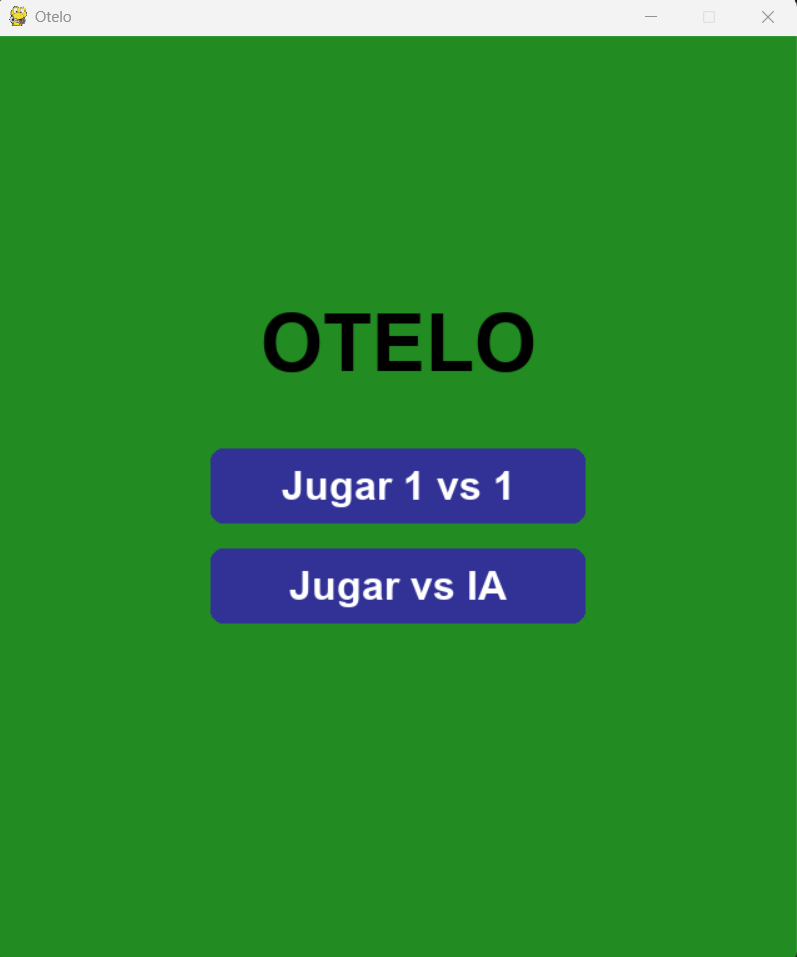
\includegraphics[width=0.85\columnwidth]{images/menu.png}
    \vspace{0.2cm}
    
    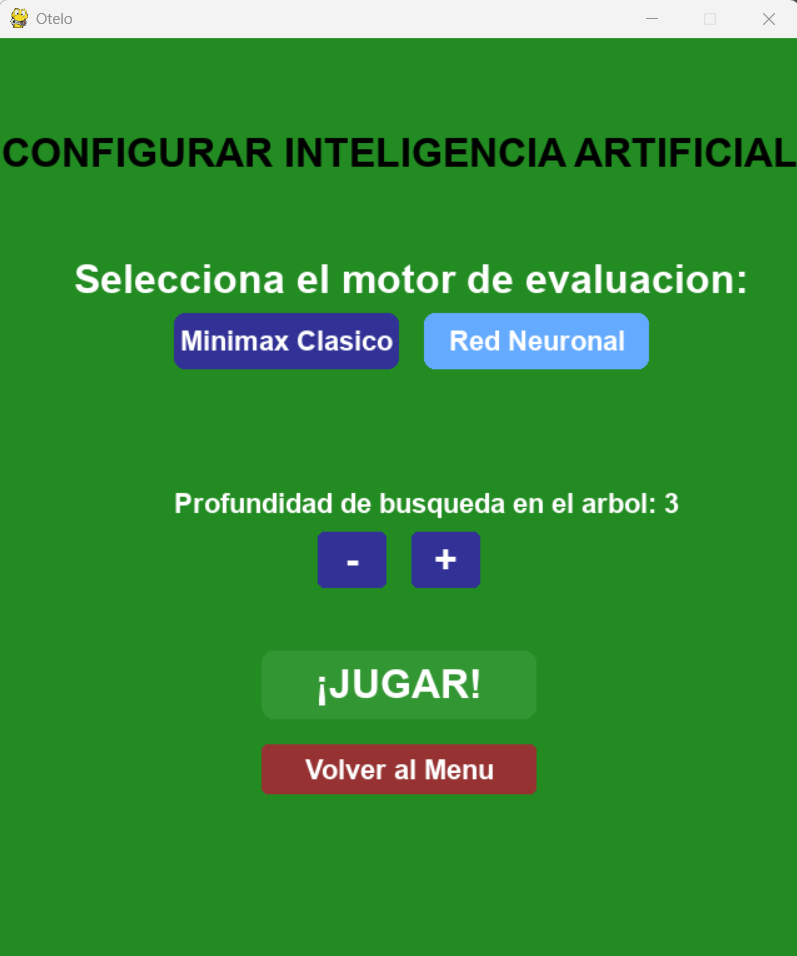
\includegraphics[width=0.85\columnwidth]{images/config.png} 
    \caption{Estados \texttt{MENU} y \texttt{CONFIG\_IA}: Flujo de inicio y parametrización de la IA.}
    \label{fig:interfaz_menu}
\end{figure}

Por otro lado, la Fig. \ref{fig:interfaz_juego} representa los estados activos del motor, mostrando la representación gráfica del tablero de $8 \times 8$, el panel de información en tiempo real y la pantalla con el resultado final una vez alcanzada la condición de victoria.

\begin{figure}[H]
    \centering
    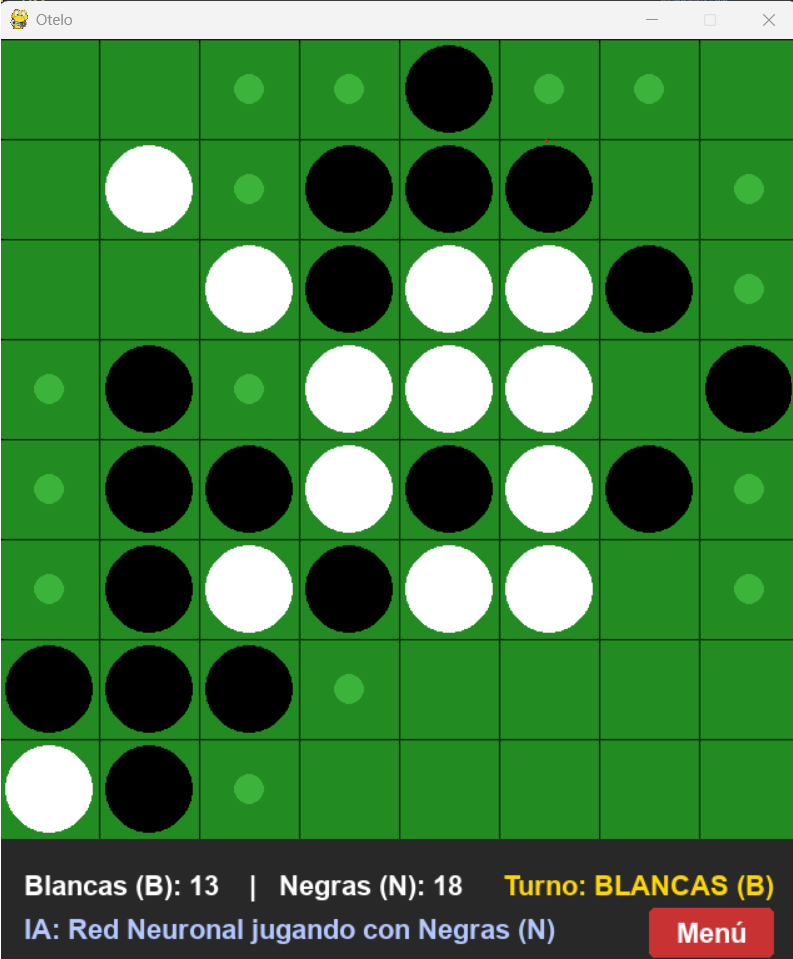
\includegraphics[width=0.85\columnwidth]{images/jugando.png} 
    \vspace{0.2cm}
    
    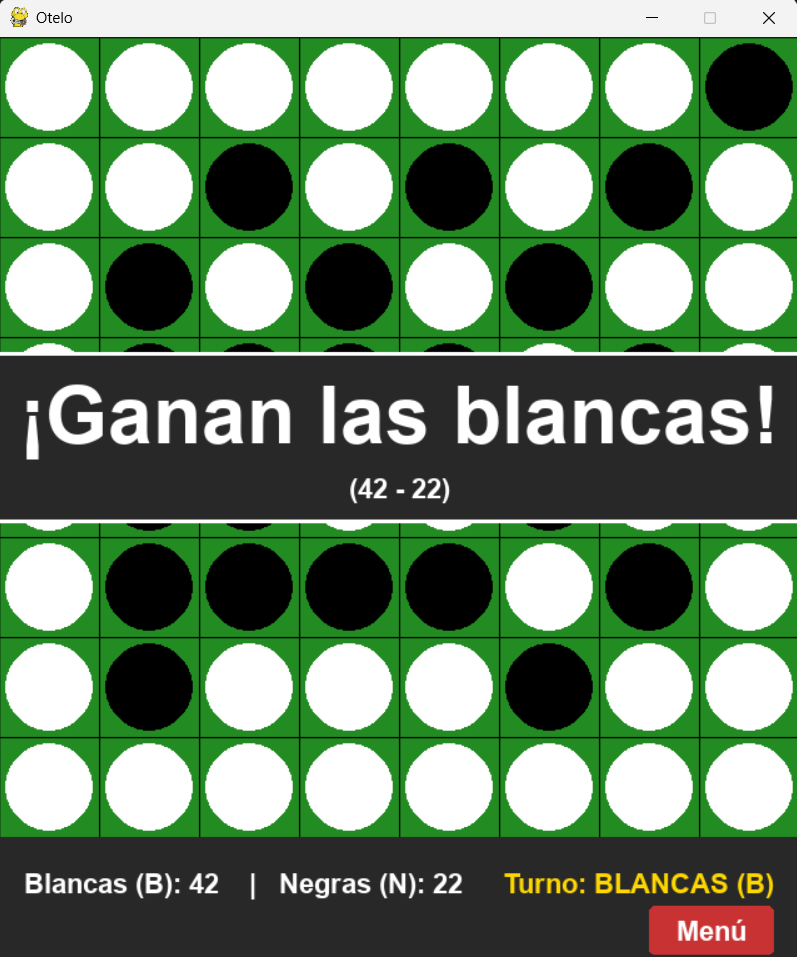
\includegraphics[width=0.85\columnwidth]{images/partida_fin.png} 
    \caption{Estados \texttt{JUGANDO} y \texttt{FIN}: Renderizado en tiempo real y resolución de la partida.}
    \label{fig:interfaz_juego}
\end{figure}


\section{Pruebas y experimentación}
\subsection{Estudio de Hiperparámetros y Selección del Modelo}
Con el objetivo de optimizar la capacidad de generalización del modelo, en la fase de pruebas no se entrenó un único modelo, sino que se realizó un estudio comparativo evaluando
tres \textbf{configuraciones distintas de hiperparámetros}.\\ 

Para garantizar la equidad, se mantuvo la semilla de pseudoaleatoriedad, asegurando que el reparto del 20\% de los datos de prueba fuera idéntico para todos los candidatos. 
Los tres modelos evaluados, todos con una estructura de 64 y 32 neuronas    en sus capas ocultas, fueron los siguientes:\\
\begin{itemize}
    \item \textbf{Modelo A (Base)}: Arquitectura base con función de activación \textit{ReLu} y optimizador \textit{SGD} con tasa de aprendizaje de 0.01.
    \item \textbf{Modelo B}: Mismo optimizador, pero sustituyendo \textit{ReLu} por la función de activación \textit{Sigmoide} en las capas ocultas.
    \item \textbf{Modelo C}: Arquitectura base (\textit{ReLu}), pero sustituyendo el optimizador clásico por el algoritmo \textit{Adam} con tasa de aprendizaje de 0.001, buscando
    una convergencia más rápida y estable.\\
\end{itemize}

Tras someter a los tres modelos a 50 épocas de entrenamiento, los resultados del error absoluto medio (MAE) sobre el conjunto de validación fueron los siguientes:
\begin{itemize}
    \item \textbf{Modelo A (Base)}: MAE de 0.9846.
    \item \textbf{Modelo B (Sigmoide)}: Logró el mejor rendimiento relativo con un MAE de \textbf{0.9816}.
    \item \textbf{Modelo C (Adam)}: MAE de 1.003\\
\end{itemize}

El \textbf{Modelo C} experimentó un fenómeno de \textbf{sobreajuste}, con un error de validación superior al de entrenamiento (0.9536), lo que indica que el optimizador \textit{Adam} no fue capaz 
de generalizar adecuadamente en este caso. Por otro lado, el \textbf{Modelo B} mostró una ligera mejora respecto al modelo base. No obstante, el error cercano a 1.0 sugiere que
la red no está aprendiendo patrones significativos y, ante la duda, tiende a predecir la situacion del tablero como un empate (0).\\

Como prueba final para descartar que el error del modelo se debiera a una falta de capacidad paramétrica o a un entrenamiento demasiado corto, se diseñó un experimento 
límite (\textbf{Modelo D}). Se construyó una topología masiva con capas densas de 128, 64 y 32 neuronas, incluyendo capas de \textit{BatchNormalization} y \textit{Dropout}, y se extendió el entrenamiento hasta las 500 épocas. \\

Los resultados del Modelo D confirmaron el diagnóstico previo: la red alcanzó 
un error de entrenamiento bastante mejor que los previos (MAE de 0.8543), pero falló drásticamente en el conjunto de validación, disparando su error hasta 1.0038. Este comportamiento 
evidencia otro caso de \textbf{sobreajuste}. Al carecer de visión geométrica por el aplanado de los datos, y al tener tanta capacidad de memoria, la red optó por memorizar los tableros 
exactos del entrenamiento, perdiendo toda capacidad de generalizar reglas estratégicas. \\

El cuello de botella de todas estas arquitecturas reside en la capa de entrada \texttt{Flatten}. Al aplanar la matriz bidimensional de $8 \times 8$ a un vector de 64 elementos, 
se destruyen por completo las relaciones espaciales y geométricas de las fichas (como diagonales y adyacencias), las cuales son fundamentales para entender la mecánica 
del \textit{flanqueo}. Esta limitación técnica justifica la necesidad de evolucionar el modelo hacia arquitecturas capaces de procesar información espacial.\\

A pesar de esta limitación, el \textbf{Modelo B} demostró ser la aproximación más estable y fue seleccionado como el modelo definitivo (\texttt{otelo\_B.keras}) para competir en el torneo final.

\subsection{Torneo Final: IA Clásica vs IA Híbrida}
Una vez seleccionado el \textbf{Modelo B} como la red neuronal con mayor capacidad de generalización del estudio empírico, 
se procedió a evaluar su rendimiento en un entorno de juego real. Para ello, se diseñó un módulo de competición (\texttt{torneo.py}) capaz de enfrentar de forma automatizada 
a dos agentes diferentes.\\

El objetivo de este experimento es medir empíricamente el impacto de sustituir la heurística manual estática por la red neuronal. Los 
contendientes configurados fueron:\\
\begin{itemize}
    \item \textbf{Agente Clásico}: Implementación de Minimax con poda alfa-beta utilizando la heurística manual de conteo de fichas.
    \item \textbf{Agente Híbrido}: Implementación de Minimax con poda alfa-beta, pero reemplazando la heurística manual por la red neuronal entrenada (\texttt{otelo\_B.keras}).\\
\end{itemize}

Ambos agentes se configuraron con una profundidad máxima de búsqueda de 3 niveles. Para garantizar la equidad del enfrentamiento y mitigar la ventaja del primer movimiento, el torneo 
constó de 100 partidas consecutivas, garantizando que cada agente jugara 50 partidas con las fichas negras y 50 con las blancas.\\

Los resultados finales del torneo arrojaron un total de \textbf{75} victorias para el Agente Clásico, \textbf{24} victorias para el Agente Híbrido y \textbf{1} empate.

\begin{lstlisting}[language=Python, caption={Resultado del script de evaluación del torneo.}, label={lst:resultado_torneo}]
RESULTADOS FINALES DEL TORNEO:
    Victorias RED: 24
    Victorias CLASICO: 75
    Empates: 1
\end{lstlisting}

Este restultado es matemáticamente coherente con el análisis de la función de pérdida realizado en la sección anterior. Al carecer de una topología espacial y presentar un Error Absoluto 
Medio (MAE) cercano a 1.0, la red neuronal de la IA Híbrida sufre de un alto grado de incertidumbre al evaluar tableros en fases tempranas y medias del juego, convergiendo a 
menudo hacia \textbf{predicciones conservadoras}. Esto le otorga una desventaja táctica frente al Agente Clásico, cuya heurística manual (maximizar la diferencia de fichas) es determinista, 
está exenta de ruido algorítmico y resulta sumamente agresiva a bajas profundidades de exploración.\\

No obstante, el hecho de que el Agente Híbrido haya logrado asegurar 24 victorias (prácticamente un cuarto de las partidas) contra un oponente de naturaleza puramente determinista y 
matemáticamente optimizada constituye un hito fundamental para el proyecto. Este rendimiento demuestra que la red neuronal no está seleccionando ramas del árbol 
de decisión al azar. A pesar de sus limitaciones arquitectónicas, el perceptrón multicapa ha logrado inferir e interiorizar \textbf{patrones estratégicos} basándose exclusivamente en la observación de los datos de autojuego. \\

En definitiva, estos resultados validan de forma práctica la \textbf{viabilidad de la hibridación}, demostrando que es posible sustituir el conocimiento experto codificado 
manualmente por aproximaciones paramétricas basadas en aprendizaje profundo dentro de sistemas de búsqueda adversaria.\\

\section{Conclusiones y Trabajo Futuro}

\subsection{Conclusiones}
En este proyecto se ha diseñado, implementado y validado un sistema híbrido para el juego de tablero Otelo, logrando integrar con éxito algoritmos de \textbf{búsqueda 
adversaria clásica} con modelos de \textbf{aprendizaje profundo supervisado}. La arquitectura modular desarrollada ha permitido aislar completamente las reglas del 
motor de juego de las interfaces gráficas, facilitando tanto la interacción en tiempo real mediante una máquina de estados estricta en \texttt{PyGame} como 
la ejecución síncrona de simulaciones masivas por consola.\\

A través del estudio de hiperparámetros, se constató que el Perceptrón Multicapa (MLP) presenta limitaciones estructurales severas para aproximar 
la función heurística del tablero de Otelo. El uso de la capa de aplanado (\texttt{Flatten}) destruye las relaciones geométricas y de adyacencia de las piezas, provocando un 
rápido \textbf{sobreajuste en topologías complejas} o un estancamiento en la \textbf{predicción de empates} en topologías simples.\\ 

A pesar de este cuello de botella matemático, la validación en el torneo automatizado demostró la viabilidad práctica del agente híbrido. Lograr un 24\% de victorias 
contra un oponente Minimax puramente determinista y optimizado certifica que la red neuronal consiguió deducir e interiorizar patrones estratégicos funcionales (como el control de 
bordes y la protección de esquinas) a partir de la mera observación estadística del autojuego, validando la hipótesis central de la investigación.

\subsection{Trabajo Futuro}
La culminación de este trabajo abre \textbf{dos líneas de investigación} claras y de gran relevancia en el estado del arte de la Inteligencia Artificial, orientadas a mitigar 
las limitaciones computacionales y heurísticas identificadas durante el proyecto:

\begin{enumerate}
    \item \textbf{Transición hacia Redes Neuronales Convolucionales (CNN)}: Para solucionar la pérdida de información espacial provocada por el Perceptrón Multicapa, el 
    siguiente paso natural es tratar el tablero como una imagen bidimensional utilizando capas convolucionales (\texttt{Conv2D}). Al aplicar \textbf{filtros locales} (por ejemplo, 
    de dimensiones $3 \times 3$), el modelo será capaz de evaluar simultáneamente el estado de una casilla junto a sus ocho vecinas. Esto permitirá abstraer de forma matemática y 
    geométrica las diagonales y vectores de flanqueo, replicando la metodología estructural que llevó al éxito a sistemas históricos como AlphaGo \cite{goodfellow}.\\
    
    \item \textbf{Entrenamiento por Refuerzo mediante Autojuego Iterativo}: Para superar el problema de asignación de crédito (\textit{Credit Assignment Problem}) derivado 
    del ruido en las etiquetas absolutas de los datos de Minimax clásico, se propone implementar un ciclo de \textbf{aprendizaje iterativo autorregulado}.\\ 
    
    Bajo este enfoque, el mejor 
    modelo de red neuronal obtenido se pondría a competir contra sí mismo en miles de partidas de autojuego en segundo plano. Los estados de estas nuevas partidas, evaluados 
    con mayor madurez estratégica, se utilizarían como un conjunto de datos refinado para entrenar a una nueva generación de la red.\\ 
    
    Este proceso iterativo de coevolución, inspirado 
    en algoritmos modernos de aprendizaje por refuerzo, permitiría al agente descubrir tácticas complejas de forma completamente autónoma y libre de sesgos humanos o heurísticas manuales simplistas.
\end{enumerate}


\section{Uso de Inteligencia Artificial Generativa}
En cumplimiento con las directrices académicas sobre integridad y transparencia, se declara el uso de herramientas de Inteligencia Artificial 
generativa durante el desarrollo de este Trabajo. Las herramientas han actuado exclusivamente como 
un sistema de asistencia y tutorización bajo supervisión constante, aplicándose en los siguientes ámbitos:

\begin{itemize}
    \item \textbf{Asistencia en Ingeniería del Software y Refactorización}: Resolución de bloqueos técnicos específicos, como la congelación del 
    hilo principal de renderizado en \texttt{PyGame} y la optimización del control de eventos dentro de la Máquina de Estados Finita (FSM). 
    \textit{Ejemplo de prompt: "Cuando la IA mueve en mi bucle principal de PyGame, el texto de la pantalla desaparece hasta que me vuelve a tocar. ¿Cómo soluciono este problema de refresco?"}\\
    
    \item \textbf{Análisis Analítico de Hiperparámetros}: Apoyo en la interpretación de los datos de validación arrojados por \texttt{Keras} (MAE y Loss) para 
    diagnosticar fenómenos matemáticos como el sobreajuste (\textit{overfitting}) de la red neuronal. 
    \textit{Ejemplo de prompt: "He entrenado un modelo denso con las siguientes características: ... y he obtenido un MAE de entrenamiento de 0.85 pero un MAE de validación de 0.99. ¿Por qué ocurre este comportamiento?"}\\
    
    \item \textbf{Formato y Estilo Académico}: Asistencia en la composición tipográfica avanzada mediante \LaTeX, generación de estructuras de tablas y refinamiento del 
    tono académico en apartados teóricos. 
    \textit{Ejemplo de prompt: "Revisa la redacción de este párrafo sobre las Redes Convolucionales para asegurar que el tono sea adecuado para un artículo de estilo IEEE, comentándome qué cambios se podrían realizar."}
\end{itemize}

Cabe destacar que todo el código fuente ejecutable, la orquestación de la arquitectura del proyecto, la ejecución empírica de 
los torneos, así como las decisiones finales de diseño, son fruto del trabajo directo y exclusivo del autor de este documento.

\section{Bibliografía}

\begin{thebibliography}{00}
    \bibitem{russell} S. Russell and P. Norvig, \textit{Artificial Intelligence: A Modern Approach}, 4th ed., Pearson, 2020, ch. 5, ``Adversarial Search''.
    \bibitem{otelo_rules} World Othello Federation, ``Othello Rules,'' [Online]. Disponible en: https://www.worldothello.org/about/about-othello/othello-rules
    \bibitem{goodfellow} I. Goodfellow, Y. Bengio, and A. Courville, \textit{Deep Learning}, MIT Press, 2016.    
    \bibitem{apuntes_nn} Dpto. de Ciencias de la Computación e Inteligencia Artificial, ``Redes neuronales'', Universidad de Sevilla, Apuntes de la asignatura Inteligencia Artificial, Curso 2025/2026.
    \bibitem{alphago} D. Silver et al., ``Mastering the game of Go with deep neural networks and tree search,'' \textit{Nature}, vol. 529, no. 7587, pp. 484-489, 2016.
    \bibitem{pygame} Pygame Community, ``Pygame: a primer on game programming in Python,'' [Online]. Disponible en: https://www.pygame.org/docs/
    \bibitem{numpy} C. R. Harris et al., ``Array programming with NumPy,'' \textit{Nature}, vol. 585, no. 7825, pp. 357--362, 2020.
    \bibitem{keras} F. Chollet et al., ``Keras,'' 2015. [Online]. Disponible en: https://keras.io
    \bibitem{scikit-learn} F. Pedregosa et al., ``Scikit-learn: Machine Learning in Python,'' \textit{Journal of Machine Learning Research}, vol. 12, pp. 2825--2830, 2011.
\end{thebibliography}    

\end{document}
